x\documentclass[12pt]{article}

% set margins and spacing
\addtolength{\textwidth}{1.3in}
\addtolength{\oddsidemargin}{-.65in} %left margin
\addtolength{\evensidemargin}{-.65in}
\setlength{\textheight}{9in}
\setlength{\topmargin}{-.5in}
\setlength{\headheight}{0.0in}
\setlength{\footskip}{.375in}
\renewcommand{\baselinestretch}{1.0}
\linespread{1.0}

% load miscellaneous packages
\usepackage{csquotes}
\usepackage[american]{babel}
\usepackage[usenames,dvipsnames]{color}
\usepackage{graphicx,amsbsy,amssymb, amsmath, amsthm, MnSymbol,bbding,times, verbatim,bm,pifont,pdfsync,setspace,natbib}

% enable hyperlinks and table of contents
\usepackage[pdftex,
bookmarks=true,
bookmarksnumbered=false,
pdfview=fitH,
bookmarksopen=true,hyperfootnotes=false]{hyperref}

\begin{document}
\title{Development}
% Add a fourth name if you have four team members; fill in at least first names below
\author{Lucia Rios-Luy\thanks{lirioslu@syr.edu} \and Meghavarshini Iska\thanks{meiska@syr.edu} \and Sergio Sotelo\thanks{spsotelo@syr.edu}\and Filippo Dona'\thanks{fadona@syr.edu}}
\date{\vskip-.1in \today}
\maketitle

\vskip.3in

\section{Research Question} \label{sec:question}

How has the link between manufacturing employment and economic growth evolved over time and space?

\section{Data Overview} \label{sec:literature}
The Our World in Data chart data gives us an overview of the different world indicators that estimate the position of each country's economy and development projection. Each data point is supposed to help show how manufacturing employment and economic growth rates have changed over the years using indicators for each country. Two variables, "Manufacturing jobs as a share of total employment" and "GDP per Capita," were sectioned into developing and developed to observe the effects of manufacturing employment on developing and developed countries' growth rates. 

\subsection{Data Set (Our World in Data Chart Data)}

The Our World in Data chart dataset has been sourced from international organizations, national statistical agencies, and multiple surveys that cover social, economic, and environmental indicators for nearly all countries from 1990 to the present day. It includes over a hundred variables, but the most important ones are GDP per capita and Manufacturing jobs as a share of total employment, which offer a detailed insight into development trends on a global scale. The number of variables and observations varies depending on the year, with data provided for up to 20,000 country-year combinations across more than one indicator. This data is crucial for policymakers as it offers critical insights and long-term patterns for development across different regions of the world. 





\section{Data Acquisition}
\label{sec:theory}


    \subsection{Data Acquisition 1 (Our World in Data - Manufacturing jobs as a share of total employment)}
    
Open the web browser, navigate to the Our World in Data website, \href{https://github.com/ecn310/course-project-development/issues/12}{Github folder} and click on the "Resources" section. Look up the first variable, "Manufacturing jobs as a share of total employment," Bank World Development Indicators Data Bank page. Once the variable has been selected, choose the chart view, deselect all the pre-opted categories, and choose the "GDP per capita" filter in the "sort by" field. For our purposes, we have taken that any country with a GDP per Capita equal to or greater than 20,000 USD will be considered a developed country and below as developing. Once the data is categorized, manually select all countries, then click on the download, clicking on the "Data" option before downloading the data set completely. 
\begin{enumerate}
\item Under "Quick download" select "Download displayed data" 

\item Under "Data API" copy the "Data URL (CSV format)" 

\end{enumerate}

Below these sections are code examples that are useful for importing that data, depending on the language used. We followed the last example, using Stata to process our data. The replication package is further code. 

    \subsection{Data Acquisition 2 (Our World in Data - GDP per Capita)}
Since the data for the second "GDP per Capita" was on the same site, it was logical to follow the same steps that were implemented to get the data for variable one. 

All data links are stored in the \href{https://github.com/ecn310/course-project-development/issues/15#issuecomment-2486305999}{Github issues section of "Re-tracking"} 



\section{Data Manipulation}
\label{sec:data}

To prepare the data for an accurate analysis, we plan to follow a series of standardized steps on which we can expand on subsequently. Firstly, we import the data in Stata from Our World in Data. We then check for outliers using the command "codebook" to verify the integrity of the data, either replacing the missing information with a known value or, if this is not available, deleting the variable from our dataset.  For OWD data, we reshaped it wide to long for easier interpretation and to identify the right values as our variables, we also took out the year 2020 as it caused some discrepancy to our data due to missing information during Covid. 
The data set is integral, in order for us to tabulate certain variables for improved readability and to form initial causal links. We are working with variables, such as GDP, and manufacturing employment within the data set. A correlation test will be conducted to compare developing to developed countries and economies, and we will graph our two main variables, GDP and manufacturing employment. In a comparative analysis, we would use "codebook" to establish how often a variable is present in a dataset, and also to be able to derive and analyze the mean, median, and standard variation.



\href{https://github.com/ecn310/course-project-development/blob/main/WDI.do}{Data do-file} 


Specifically to OWD data, we must first deselect all, and then select to include all countries across all available years, and only the variables listed in the Key variables listed below for Data Set: GDP and manufacturing employment. Once the Excel file has been downloaded, we import it into Stata and proceed to reshape it for easier interpretation. Steps to follow to reshape the data can be found here: \href{https://github.com/ecn310/course-project-development/blob/main/WDI.do}{Data do-file}.
Once the data has been reshaped, it can be downloaded as a dta file. Note that should you wish to include more variables, the steps to follow in Stata remain largely unaltered, but other variables must be selected prior to downloading the spreadsheet from the OWD website. 


\section{Linking Datasets}
\label{sec:discussion}

\subsection{Data Preparation and Cleaning}

\begin{enumerate}

\item     Classifying Countries}:  
    Countries were categorized into "developed" and "developing" economies using OWD’s income-related indicators so we could perform comparative analyses between countries at these different stages of economic development.
\end{enumerate}

    \item \textbf{Importing and Reshaping the Data}:  
    The OWD dataset was imported into Stata in wide format. Using the \texttt{reshape} command, the dataset was transformed into long format, allowing efficient handling of country-year observations for longitudinal analysis.

    \item \textbf{Excluding Incomplete Observations}:  
    Observations for the year 2020 were excluded due to significant missing data caused by the COVID-19 pandemic. Additionally, any observations with missing values for "Manufacturing jobs as a share of total employment" or "GDP per capita" were removed to ensure accurate statistical analysis.

    \item \textbf{Standardizing Country-Year Identifiers}:  
    The dataset was reviewed to ensure consistency in country names and time periods. Any discrepancies in country identifiers were corrected to align observations across the variables. Only complete observations with valid country-year data were retained.

\b{enumerate}

\subsection{Data Integration and Analysis}

\begin{itemize}
    \item \textbf{Descriptive Statistics}:  
    Summary statistics, including mean, median, and standard deviation, were calculated for the two variables. These statistics were segmented by country classification (developed or developing) using Stata's \texttt{summarize} command. The analysis revealed:
    \begin{itemize}
        \item \textbf{Developing Countries}:  
     \begin{figure}
         \centering
         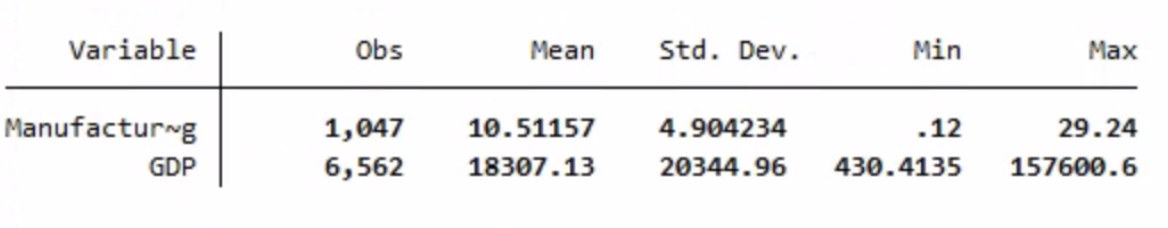
\includegraphics[width=1\linewidth]{Screenshot 2024-12-02 at 9.41.32 AM.png}
         \caption{Enter Caption}
         \label{fig:enter-label}
     \end{figure}
      \end{figure}

        \item Developed Countries:  
\begin{figure}
        \centering
        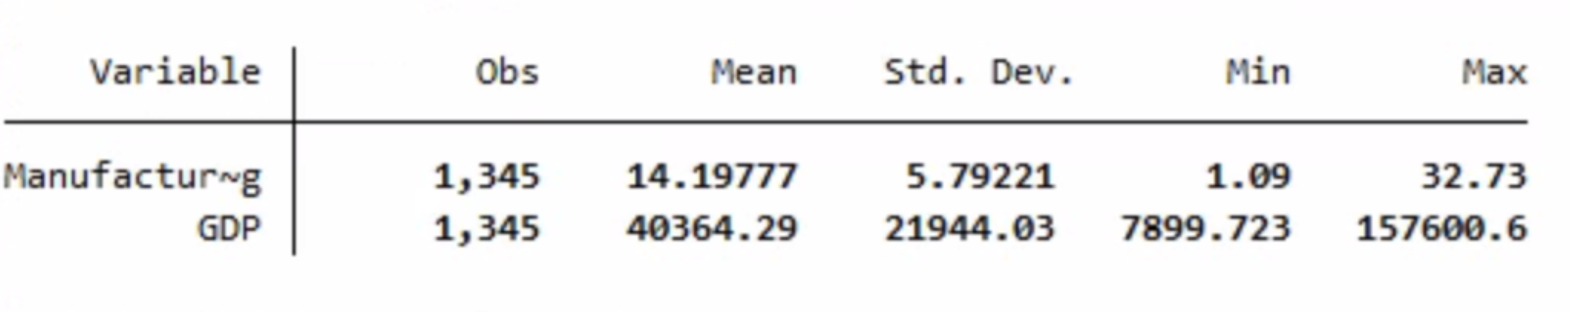
\includegraphics[width=1\linewidth]{Screenshot 2024-12-02 at 9.40.49 AM.png}
        \caption{Enter Caption}
        \label{fig:enter-label}
    \end{figure}
        \end{itemize}

    \item \textbf{Correlation Analysis with p-values}:  
    A correlation analysis was performed using Stata’s \texttt{pwcorr} command with the {sig} option to calculate correlation coefficients and p-values. Results indicated:
    \begin{itemize}
        \item In developed countries, a weak negative correlation (\(r = -0.36\), p-value < 0.001) suggested that as manufacturing employment declines, GDP tends to rise, reflecting shifts toward service-based industries.
        \item In developing countries, a moderate positive correlation (\(r = 0.28\), p-value < 0.05) supported the hypothesis that manufacturing employment drives GDP growth, emphasizing its role in industrialization and export-led production.
    \end{itemize}

    \item \textbf{Graphical Analysis}:  
  The following line graphs were created to visualize trends in GDP per capita and manufacturing employment over time for both developed and developing countries. These graphs span from 1990 to 2022 and exclude data for the year 2020 due to significant disruptions caused by the COVID-19 pandemic.
  
\begin{itemize}
    \item "As shown in Figure 1, the GDP per capita for developing countries has grown steadily, reflecting economic progress, while manufacturing trends (Figure 2) demonstrate variability but remain critical to economic output."
    \item The decline in manufacturing share (Figure 4) illustrates the shift towards service-oriented economies, while GDP trends (Figure 3) continue to show a steady upward trajectory
\end{itemize}


(Figure 1):
\begin{figure}
    \centering
    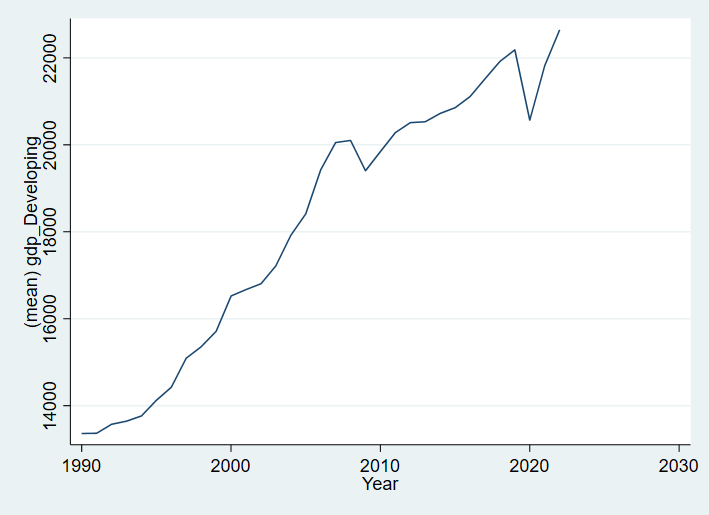
\includegraphics[width=0.75\linewidth]{391423396-9d8ae4b4-2a48-4b9f-8427-e7c3ebc5fb9f.png}
    \caption{GDP per capita trends for developing countries (1990–2022), showing steady growth over time.}
    \label{fig:enter-label}
\end{figure}

(Figure 2):
\begin{figure}
    \centering
    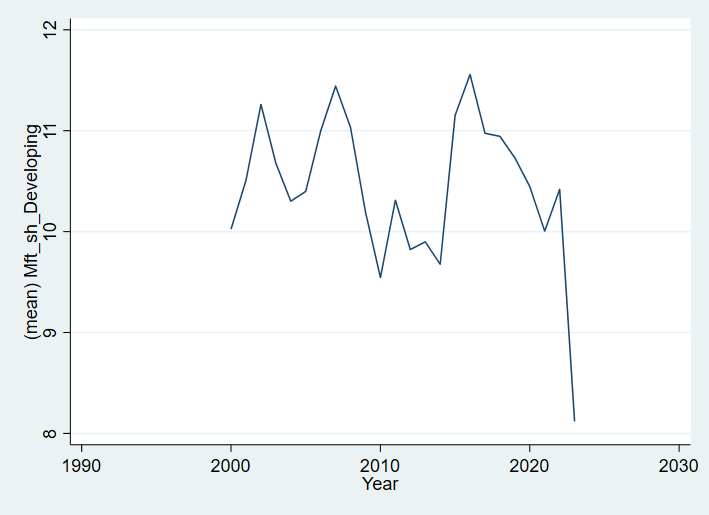
\includegraphics[width=0.75\linewidth]{391423390-5a4d719e-8e42-4cd2-9850-69f08fac8a68.png}
    \caption{Manufacturing share of employment in developing countries (1990–2022), highlighting variations and trends over the years.}
    \label{fig:enter-label}
\end{figure}

(Figure 3):
\begin{figure}
    \centering
    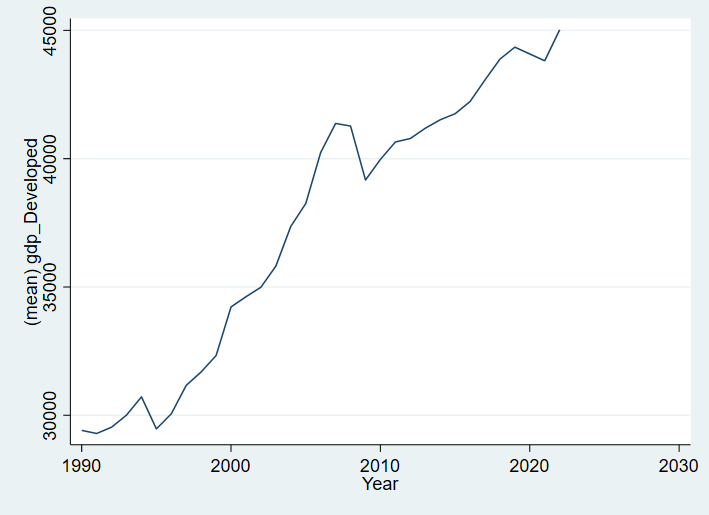
\includegraphics[width=0.75\linewidth]{DEVELOPED GDP GRAPH.png}
    \caption{GDP per capita trends for developed countries (1990–2022), showing steady growth over time)}
    \label{fig:enter-label}
\end{figure}

(Figure 4):
\begin{figure}
    \centering
    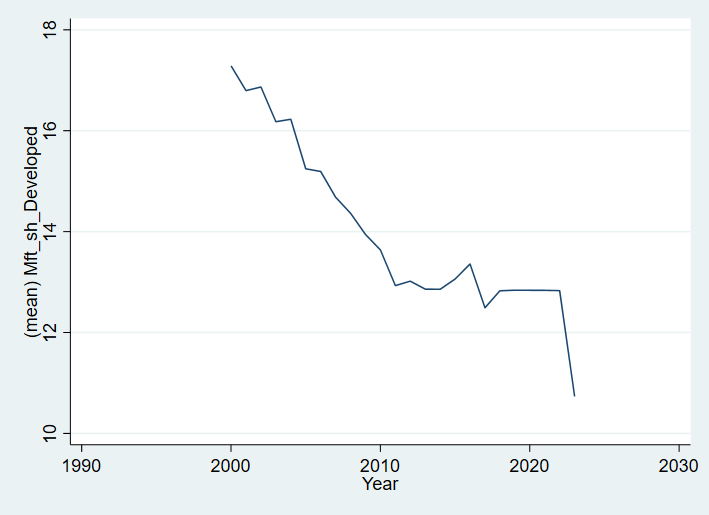
\includegraphics[width=0.75\linewidth]{391423369-a4547c99-f102-45fa-a2db-d2455b3472d00.png}
    \caption{Manufacturing share of employment in developing countries (1990–2022), highlighting a consistent decline over time, reflecting reduced reliance on manufacturing.}
    \label{fig:enter-label}
\end{figure}

\section{Key Variables}
\label{sec:result}  

\begin{enumerate}
    \item \textbf{Manufacturing Jobs as a Share of Total Employment}  

This variable reflects the role of industrial activity in a country’s economy and labor market and  provides a key measure of industrialization's contribution to economic development.
    \end{itemize}

    \item \textbf{GDP per Capita}  
    
This variable helps highlight the living standards and economic productivity across countries.

    \item \textbf{Country Classification}  
    
This variable creates comparative analysis between developed and developing economies, highlighting differences in the relationship between manufacturing employment and GDP growth.

    \item \textbf{Year}  
    
This variable allows for the analysis of trends, revealing how the relationship between manufacturing employment and GDP per capita has evolved over time.

\end{document}
